
\chapter{GNU Radio Implementation} \label{ch:GNUradio}

Traditionally, X-band satellite reception relied on expensive, fixed-function hardware. Today, Software-Defined Radio (SDR) provides a more flexible approach by shifting the core signal processing from physical integrated circuits to software algorithms. This chapter details the construction of the SDR receiver architecture—referred to throughout this report as the signal processing \textit{pipeline}\footnote{Throughout this report, the terms \textit{pipeline} and \textit{flowgraph} are used interchangeably to denote the GNU Radio architecture—a sequence of interconnected Digital Signal Processing (DSP) modules designed to transform a raw stream of digitized Radio Frequency (RF) samples into decoded telemetry.}. 

A critical constraint defining this architecture is real-time execution. Every processing stage, from Doppler estimation to $\mathtt{Viterbi}$ decoding, must be computationally efficient and perfectly synchronized. The main challenge lies not only in demodulating the signal, but in optimizing the code to process the high data rate without buffer overflows or frame loss, effectively keeping pace with the continuous RF capture.

\begin{figure}[h]
    \centering
    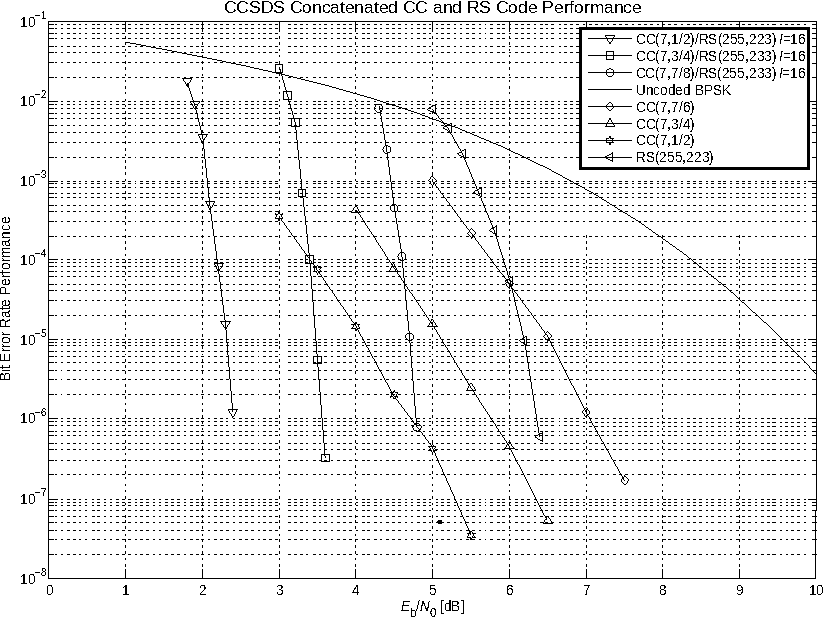
\includegraphics[width=0.7\textwidth]{figures/Inkscape/CCSDS_performance.pdf} 
    \caption{Performance of Concatenated Coding Systems with Ideal Interleaving, E=16, Punctured Codes \autocite[Figure 6-4 in]{CCSDS_130_1_G_3}.}
    \label{fig:CCSDS_performance} 
\end{figure}


\section{Design and Justification}

The \href{https://www.gnuradio.org/}{GNU Radio} community is highly active, resulting in a substantial body of open-source code that provides software-defined solutions for applications akin to the one addressed in this report. Regarding the \textsf{CCSDS} suite of protocols, several libraries have been instrumental to our work, such as \autocite[gr-satellites]{gr_satellites}, \autocite[gr-highdatarate-modem]{gr_highdatarate_modem}, \autocite[gr-ccsds]{gr_ccsds}, and the native GNU Radio blocks themselves \href{https://wiki.gnuradio.org/index.php?title=Category:Block_Docs}{(Block Docs)}. As previously established in \Cref{ch:Pipeline}, fulfilling the core objectives of this project requires evaluating the receiver against a complete \textsf{TX}-\textsf{RX} simulation chain. By leveraging these libraries, we constructed this full simulation environment to generate our \textsf{BER} curves and rigorously characterize the system's performance.

To achieve this, we utilized all the aforementioned libraries (except for \autocite{gr_ccsds}, as its blocks are outdated). The most widely adopted library is \autocite{gr_satellites}, but it primarily provides blocks for \textsf{RX}. Furthermore, during our evaluation, we found that some blocks did not perform as expected, others were only partially implemented, and a few did not strictly adhere to the standard. We will discuss a major missing implementation issue within these libraries later in \Cref{ch:Frame_sync}. Consequently, by integrating blocks from various libraries and programming new custom blocks ourselves, we successfully developed a flowgraph that operates in compliance with \textsf{CCSDS} specifications. In the appendix, you can refer to \Cref{fig:ccsds_custom}, which illustrates the blocks we programmed alongside those reused from existing libraries. These custom blocks can be found in the following library \href{https://tclgit.epfl.ch/semester-projects/26s-pereirariquelme-sdr-xband-receiver}{SDR-Xband-receiver}.

It is worth noting that the simulations found in the \textsf{CCSDS} documentation represent ideal performance curves. According to the information provided in the \(\mathcal{G}reen\) \(\mathcal{B}ooks\), the performance depicted in \Cref{fig:CCSDS_performance} assumes an \textsf{AWGN} channel, perfect symbol and frame synchronization, and an ideal pulse-shaping filter. These assumptions are made to demonstrate the maximum theoretical capability of these mathematical codes.

\begin{figure}[h]
    \centering
    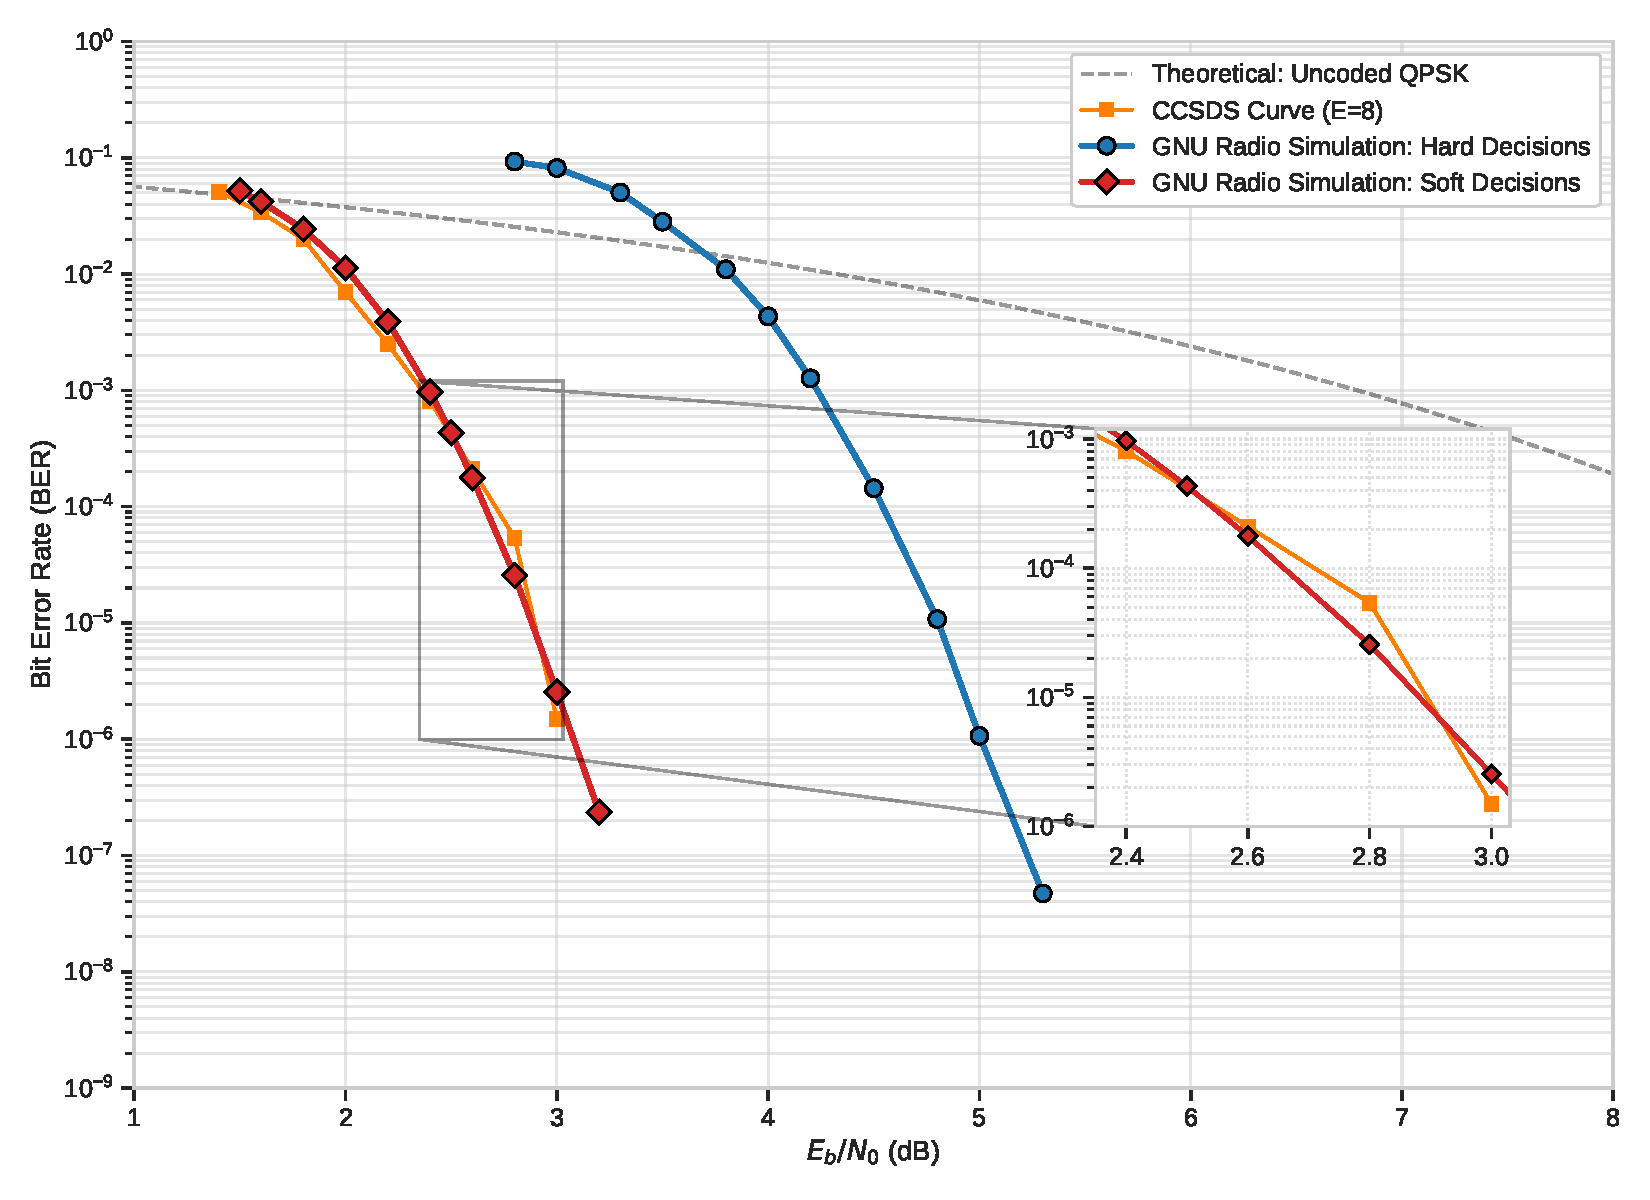
\includegraphics[width=1\textwidth]{figures/Inkscape/Sync_BER_Comparison_with_CCSDS.pdf} 
    \caption{Simulated curve in GNU Radio vs. CCSDS curve found in \autocite[Figure 6-9]{CCSDS_130_1_G_3} for an Interleaving Depth of 1 and E=8.}
    \label{fig:CCSDS_performance_sim} 
\end{figure}

Taking this into account, we simulated the system to obtain \Cref{fig:CCSDS_performance_sim} and observed that our result is practically identical to the standard's theoretical curve. In fact, our curve appears smoother, likely due to the higher number of simulated frames. Additionally, we plotted the system's performance assuming hard decisions to serve as a baseline. As established in classical communication theory, hard-decision decoding typically introduces a performance degradation of approximately 2 dB compared to unquantized soft decisions. However, this plot is strictly illustrative; our final receiver architecture exclusively employs soft-decision decoding to maximize the coding gain.

However, these ideal graphs are insufficient to evaluate the practical implementation of the receiver. In the subsequent chapters, we will introduce a complete channel simulation model to examine the operational challenges of the link. Specifically, we will analyze the impact of the Doppler effect and demonstrate how to develop a robust algorithm to solve the frame synchronization problem. By integrating these physical impairments and their respective tracking mechanisms into the simulation, we will generate more realistic BER curves. As we incorporate Doppler compensation and real-time frame synchronization, the BER will naturally increase when compared to the purely ideal curves simulated previously.


